\subsection{Dataset preparation} \label{sec:dataset}
As mentioned in the introduction, there were no off-the-shelf thermal multispectral datasets available for training and testing our proposed method.
The only remotely related available datasets were of satellite missions, but those are not open-sourced and only provide post-processed data (\eg, estimated humidity) maps rather than raw thermal images.
Therefore, we assembled a dedicated dataset in-house using a light airplane equipped with the same camera that was used to calibrate the physical model (FLIR Tau2).
The pilot performed several flights, with a $9 \mu m$ IR bandpass filter applied to the camera lens (which we refer to as \emph{monochromatic} images), or without this filter (which we refer to as \emph{panchromatic} images).

Ensuring that the plane trajectory and camera position are the same for two different flights is physically infeasible. Therefore, the monochromatic and panchromatic sets are necessarily unpaired.
This guided us toward basing our method on an UI2I translation model as described in section \ref{sec:methods}.

\subsection{Metrics}
Since our dataset is unpaired, pixel-based metrics are not fit for performance evaluation. 
This implies that only statistically based metrics are viable.
One such metric is the Fréchet Inception Distance (FID) \cite{DBLP:journals/corr/HeuselRUNKH17}, which is widely used for evaluating the quality of generated images and specifically GANs.
Typically, a lower FID score indicates greater fidelity of the generated images to the real target modality.
We note here that while the density and coverage (DC) \cite{naeem2020reliable} metric is the most recent and popular approach for evaluating GANs, its coverage component is irrelevant for I2I tasks because the output's content is necessarily conditioned on the input.

One could argue that FID isn't an optimal metric of choice in our case, as the underlying network providing its score was pre-trained on RGB images rather than thermal ones.
However, as shown Oz \etal \cite{Oz:20} for super-resolution, neural networks trained with RGB data generalize very well for thermal images as well.
Following this argument, it made sense to rely on FID as a proper measure of fidelity between thermal image modalities.
Therefore, and in the absence of compellingly better alternatives, we use FID as our sole numerical evaluation metric.


\subsection{Experimental setup}
As a rule of thumb, the FID metric requires test sets of about $10,000$ images from each modality to be indicative of their true statistical distribution. 
This clearly limits the amount of data left for training and validation.
Thus, only $1000$ images were used for training and $100$ for validation per modality, resulting in a total of $2200$ images.

To fairly assess the method's contribution, we first trained our baseline models (CycleGAN, CUT) and fine-tuned their hyper-parameters and design choices.
Consequently, the following changes were made (\wrt the original implementation) to achieve optimal FID score on our dataset: 
the generator's bottleneck was implemented using 6 residual blocks (instead of 9), the learning rate was set to $5 \times 10^{-4}$ (instead of $2 \times 10^{-4}$) and a batch size of $2$ was used (instead of $1$).
In addition, we applied a statistically based input-normalization technique, \ie, the mean and standard deviation of each modality were calculated based on the entire training set, and then used to normalize all training, validation and test images.

The same set of hyper-parameters and design choices were applied as is for training all our proposed methods and their ablative configurations.
For each model configuration, FID was calculated at the end of every epoch.
The minimum (best) FID score over all epochs was treated as the score of that configuration.
We note that since the FID is an evaluation metric, it should in essence be calculated only at test time, after training has already ended. 
Nevertheless, as the hyper-parameters were prefixed for all configurations, calculating the FID score had no impact over the optimization procedure.
Therefore, there was no flaw in calculating it at the end of every epoch.

\subsection{Results}
\subsubsection{Quantitative}
Typically, numerical scores are obtained by training a network and evaluating it once.
However, due to the highly non-convex nature of the deep networks loss functions, the local minimum to which a network converges is highly dependent on its weight initialization.
The findings of \cite{picard2021torch} further illustrate that a network trained once (\ie, with a single weight initialization) can have an outlier score that is much better or much worse than the average.

Therefore, we chose a statistical approach to evaluate and compare the different configurations.
For each configuration, we trained and evaluated the FID score 10 consecutive times, where we randomly initialized the weights in every training-evaluation cycle.
We then calculated the mean and standard deviation of the 10 FID scores and used them as criteria for comparison with the other configurations.
This approach reduces the sensitivity to the randomness of the weight initialization, and provides a measure for the model's robustness \wrt random initialization, which can be inferred from the standard deviation.

The numerical comparison between the different configurations can be found in Table \ref{tbl:results}.
We tested every possible configuration of our propositions, \ie, with and without providing the intrinsic temperatures  to the deep generator, and with and without fusing the deep generator with the physical estimator.
All configurations were tested on top of both baseline models (CycleGAN and CUT).

\begin{table}
    \centering
    \begin{tabular}{| c  c  c  c || c  c |}
        \multicolumn{4}{c}{Configuration} & \multicolumn{2}{c}{FID} \\
        \hline
        Backbone & Int & Phys & Caption & Mean & Std\\
        \hline
        \multirow{4}{4em}{\centering CycleGan}  & \xmark & \xmark & Baseline    & 51.05             & 9.82\\      
                                                & \xmark & \cmark &             & 35.54             & 3.72\\ 
                                                & \cmark & \xmark &             & 50.17             & 8.89\\
                                                & \cmark & \cmark & PETIT       & \textbf{33.8}     & \textbf{1.23}\\
        \hline
        \multirow{4}{4em}{\centering CUT}       & \xmark & \xmark & Baseline    & 38.43             & 1.52\\
                                                & \xmark & \cmark &             & 29.85             & \textbf{0.99}\\
                                                & \cmark & \xmark &             & 48.88             & 1.46\\
                                                & \cmark & \cmark & PETIT       & \textbf{27.35}    & 1.01\\
        \hline
    \end{tabular}
    \caption{Comparison of FID score statistics between the different configurations (the lower the better). \emph{Int} stands for intrinsic temperature and \emph{Phys} for physical estimator.}
    \label{tbl:results}
\end{table}

PETIT was found to dominate all other configurations with both backbones.
Specifically, compared to the baseline configurations, PETIT achieved an approximately $50\%$ mean FID improvement and a significantly improved standard deviation, indicating a more robust solution.
Another interesting observation was that all configurations involving the physical estimator outperformed their counterparts by a large margin, in terms of both mean and standard deviation.
On the other hand, the intrinsic temperature information alone did not seem to have a significant impact on the results, and was only helpful when combined with the physical estimator.
This suggests that the physically estimated prior information steers the optimization procedure toward points on the manifold where the intrinsic temperature information is locally beneficial.

\subsubsection{Qualitative} \label{subsubsec:qual_res}
In accordance with the quantitative results, the monochromatic outputs produced by PETIT seem to be of superior quality compared to all other configurations.
Generally speaking, PETIT's outputs incur less spurious artifacts and exhibit stronger fidelity to real monochromatic modality. 
An impression of the discussed superiority can be obtained from the examples in Figure \ref{fig:qual_comp}.
Due to space limitations, we only display the outputs of CycleGAN and CUT baselines \vs the CUT-backbone-based PETIT configuration.
Real unpaired monochromatic images are also displayed in juxtaposition to the generated outputs for an impression of the modality's true nature.
\begin{figure*}
    % 1st Row
    \centering
    \begin{subfigure}[b]{0.19\textwidth}
        \centering
        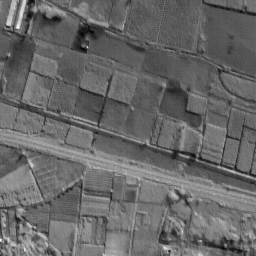
\includegraphics[width=\textwidth]{../figs/outputs/pan/71.png}
    \end{subfigure}
    \hfill
    \begin{subfigure}[b]{0.19\textwidth}
        \centering
        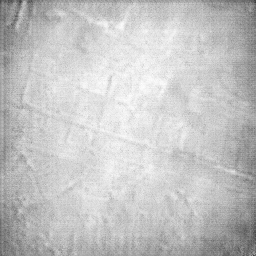
\includegraphics[width=\textwidth]{../figs/outputs/cycleGan/71.png}
    \end{subfigure}
    \hfill
    \begin{subfigure}[b]{0.19\textwidth}
        \centering
        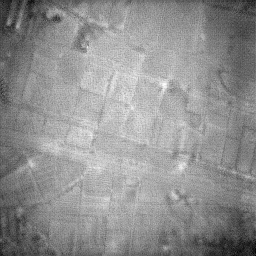
\includegraphics[width=\textwidth]{../figs/outputs/cut/71.png}
    \end{subfigure}
    \hfill
    \begin{subfigure}[b]{0.19\textwidth}
        \centering
        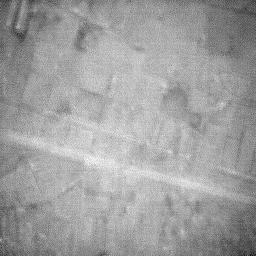
\includegraphics[width=\textwidth]{../figs/outputs/petit/71.png}
    \end{subfigure}
    \hfill
    \begin{subfigure}[b]{0.19\textwidth}
        \centering
        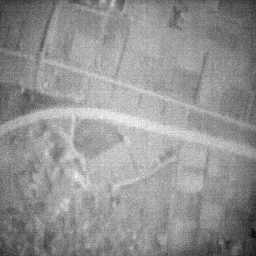
\includegraphics[width=\textwidth]{../figs/outputs/mono/605.png}
    \end{subfigure}      
    
    % 2nd Row
    \centering
    \begin{subfigure}[b]{0.19\textwidth}
        \centering
        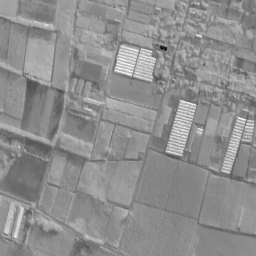
\includegraphics[width=\textwidth]{../figs/outputs/pan/24.png}
    \end{subfigure}
    \hfill
    \begin{subfigure}[b]{0.19\textwidth}
        \centering
        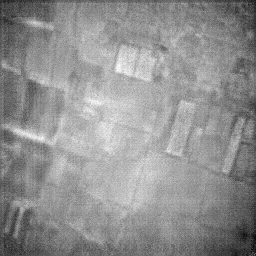
\includegraphics[width=\textwidth]{../figs/outputs/cycleGan/24.png}
    \end{subfigure}
    \hfill
    \begin{subfigure}[b]{0.19\textwidth}
        \centering
        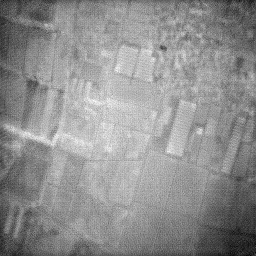
\includegraphics[width=\textwidth]{../figs/outputs/cut/24.png}
    \end{subfigure}
    \hfill
    \begin{subfigure}[b]{0.19\textwidth}
        \centering
        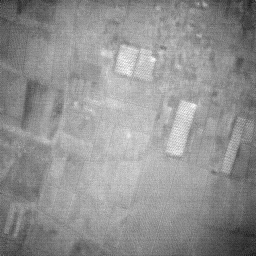
\includegraphics[width=\textwidth]{../figs/outputs/petit/24.png}
    \end{subfigure}
    \hfill
    \begin{subfigure}[b]{0.19\textwidth}
        \centering
        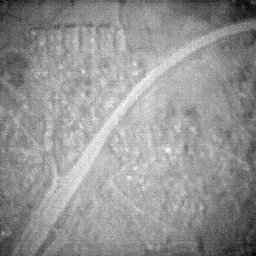
\includegraphics[width=\textwidth]{../figs/outputs/mono/508.png}
    \end{subfigure}    
    
    % 3rd Row
    \begin{subfigure}[b]{0.19\textwidth}
        \centering
        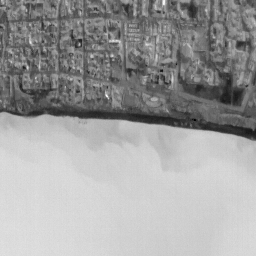
\includegraphics[width=\textwidth]{../figs/outputs/pan/28.png}
        \subcaption{Pan (input)}
        \label{fig:pan}
    \end{subfigure}
    \hfill
    \begin{subfigure}[b]{0.19\textwidth}
        \centering
        
\includegraphics[width=\textwidth]{../figs/outputs/cycleGan/28.png}
        \subcaption{CycleGAN (baseline)}
        \label{fig:cycleGan}
    \end{subfigure}
    \hfill
    \begin{subfigure}[b]{0.19\textwidth}
        \centering
        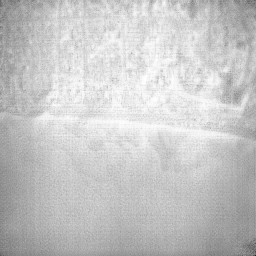
\includegraphics[width=\textwidth]{../figs/outputs/cut/28.png}
        \subcaption{CUT (baseline)}
        \label{fig:cut}
    \end{subfigure}
    \hfill
    \begin{subfigure}[b]{0.19\textwidth}
        \centering
        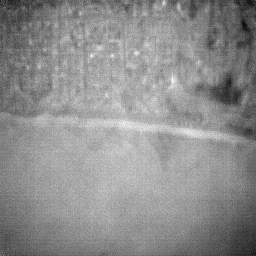
\includegraphics[width=\textwidth]{../figs/outputs/petit/28.png}
        \subcaption{PETIT (ours)}
        \label{fig:petit}
    \end{subfigure}
    \hfill
    \begin{subfigure}[b]{0.19\textwidth}
        \centering
        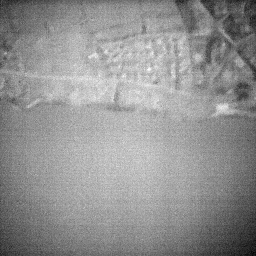
\includegraphics[width=\textwidth]{../figs/outputs/mono/994.png}
        \subcaption{Mono (ref)}
        \label{fig:mono}
    \end{subfigure}

    \caption{Qualitative comparison. (a) Panchromatic (Pan) input. (b) CycleGAN output. (c) CUT output. (d) PETIT output. (e) Real unpaired monochromatic image (Mono) for reference.}
    \label{fig:qual_comp}
\end{figure*}
For additional examples, please refer to section \ref{Supp-sec:additional_res} in the supplementary material.